\documentclass{article}
\usepackage{array}
\usepackage{graphicx}
\usepackage{lscape}
\usepackage{amsmath}
\usepackage{multirow}
\usepackage{hyperref}
\usepackage{subfig}

\usepackage[latin1]{inputenc}
\usepackage{tikz}
\usetikzlibrary{calc, shapes, arrows, positioning}

\DeclareMathOperator{\SJ}{SJ}

\renewcommand{\baselinestretch}{1.1}
\newcommand{\prog}[1]{{\tt\em #1}}

\begin{document}
\title{Splicing Analysis and Quantification Pipeline}
\author{Dmitri D. Pervouchine}
\date{\today}
\maketitle

\tableofcontents

\section{Overview}
This document contains a full description of main processing steps of splicing analysis and quantification pipelines. 
There are at least two such independent pipelines, abbreviated here as SJPIPE and TXPIPE. 

SJPIPE implements the quantification of splicing events by directly analyzing the alignments in BAM files 
(Figure~\ref{fig::sjpipe}). The advantage of SJPIPE is that it allows quantification of annotated as well as 
novel splice junctions and that there is no annotation-related interference between independent splicing events. 
An obvious disadvantage, however, is that only a part of the sequencing information is used, one which is related 
to local short read distribution at splice junctions, while the reads that are contained in exons or introns are 
completely ignored.

In SJPIPE pipeline, the BAM file is read by \prog{sjcount} utility to produce a tab delimited output of splice junction 
counts with offsets and, additionally, the respective counts of the continuous reads that overlap splice junctions 
(explained below). This output is aggregated (\prog{aggregate.pl}), matched against genome and annotation (\prog{annotate.pl}), 
and passed to strand disambiguation (\prog{choose\_strand.pl}). The resulting stranded counts are then subject to the 
irreproducibility assessment (\prog{npIDR}) and filtering (\prog{filter}). Importantly, this pipeline is designed to 
work uniformly with
\begin{itemize}
\item stranded and unstranded data
\item data with and without bioreplicates
\end{itemize}

The TXPIPE pipeline quantifies annotated splicing events by analyzing the transcript quantification data produced by some 
other program. The advantage of this approach is that it deconvolves exon abundancies by taking into account all sequencing 
data, i.e., not only the local short read distribution at splice junctions, but also the distribution of short reads in exons 
and introns. This leads to a larger effective sample size compared to that in SJPIPE. A disadvantage, however, is that an 
unannotated splicing event or a number of annotated dependent splicing events may distort the global splicing pattern significantly 
and, therefore, there is no guarantee that the inclusion rates of each given exon reflect actual splicing events that occur 
with the given exon.

\begin{figure}
\centering
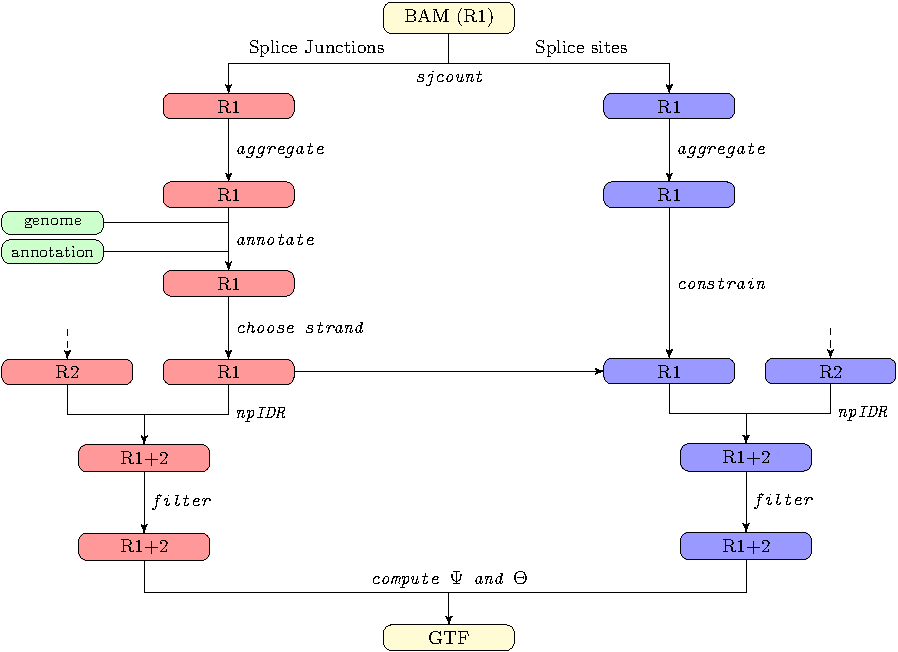
\includegraphics[width=\textwidth]{latex/fig1_crop.pdf}
\caption{The SJPIPE pipeline.\label{fig::sjpipe}}
\end{figure}


\section{Detailed description of the components}

\subsection{Pipeline generator}
The \prog{make.pl} utility takes as an input an index file and outputs to the standard output a makefile to be executed to run the pipeline.
\begin{verbatim} 
make.pl -dir <dirname> -param <params> -by <attribute> -margin 
          <length> -annot <gtf> -genome <name> -merge <name>
Inputs: -annot ..., the annotation (gtf), obligatory
        -block ..., the blocking field for mastertable
        -dir ..., the output directory, obligatory
        -entropy ..., entropy lower threshold, default=3
        -genome ..., the genome (without .dbx or .idx), obligatory
        -group ..., the grouping field for IDR, obligatory
        -idr ..., IDR upper threshold, default=0.1
        -margin ..., margin for aggregate, default=5
        -merge ..., the name of the output to merge in case if blocks are missing
        -mincount ..., min number of counts for the denominator, default=20
        -param ..., parameters passed to sjcount
        -repository ..., the repository subdirectory for bam files
        -status ..., annotation status lower threshold, default=0
        STDIN:  an index file 
Output: STDOUT: a GNU MAKE makefile
        make -f file.mk all
\end{verbatim} 

For example, the command
\begin{verbatim}
make.pl -dir data/human/ -param '-read1 0 -read2 0' -margin 4 
          -annot hg19v10.gtf -genome genome/homSap19 
          -group labExpId -block rnaExtract < index.txt > pipeline.mk
\end{verbatim}
creates a file called 'pipeline.mk' based on the input from 'index.txt', where all the intermediate steps will be stored in 'data/human/' (needs 
to created beforehand), with the annotation file hg19v10.gtf in the current directory, and with genome/homSap19.idx and genome/homSap19.dbx both 
being readable files. The master tables will be named data/human/output*.tsv

%%%%%%%%%%%%%%%%%%%%%%%%%%%%%%%%%%%%%%%%%%%%%%%%%%%%%%%%%%%%%%%%%%%%%%%%%%%%%%%%%%%%%%%%%%%%%%%%%%%%%%%%%%%%%%%%%%%%%%%%%%%%%%%%%%%%%%%%%%%%%%%

\subsection{Pre-processing}

\subsubsection{Annotation pre-processing}
\label{sec::preprocessing}

Genomic annotation files usually come in gtf format and contain many feature types. Often these are large files and it takes time to read such a file. 
Sometimes they may be incomplete (e.g. contain exons, but not introns). The \prog{transcript\_elements.pl} utility reads such a gtf, extracts only
exons and transcript identifiers, to which these exons belong, and outputs a shorter form of gtf which contains (1) exons and (2) introns calculated 
based on the exon information. The format of the output is also gtf, where in the last column (column 9), the 'belongsto' attribute lists the transcripts 
to which given exon or intron belongs. For example, in the input gtf were
\begin{verbatim} 
...   ...     ...  ... ... . . . ...      
chr2L FlyBase exon 100 200 . + . gene_id "8"; transcript_id "1";
chr2L FlyBase exon 300 400 . + . gene_id "8"; transcript_id "1"; 
chr2L FlyBase exon 500 600 . + . gene_id "8"; transcript_id "1"; 
chr2L FlyBase exon 100 200 . + . gene_id "8"; transcript_id "2"; 
chr2L FlyBase exon 500 600 . + . gene_id "8"; transcript_id "2"; 
...   ...     ...  ... ... . . . ...
\end{verbatim}
then the pre-processed, shorter form would have been
\begin{verbatim} 
chr2L SJPIPE  exon    100   200   .    +    belongsto "1,2";
chr2L SJPIPE  intron  200   300   .    +    belongsto "1";
chr2L SJPIPE  intron  200   500   .    +    belongsto "2";
chr2L SJPIPE  exon    300   400   .    +    belongsto "1";
chr2L SJPIPE  intron  400   500   .    +    belongsto "1";
chr2L SJPIPE  exon    500   600   .    +    belongsto "1,2";
\end{verbatim}
Note that transcripts and introns are not shown in the input gtf. The information contained in the 'belongsto' field will be used only in 
TXPIPE pipeline to compute splicing indices from transcript quantification (see section~\ref{sec::txpipe}).

{\bf NB} In what follows, the processed annotation has to be sorted. Therefore it is necessary to pipe it with the sort step as follows.

\begin{verbatim} 
perl Perl/transcript_elements.pl - < input.gtf | sort -k1,1 -k4,5n > output.gff
\end{verbatim}

%%%%%%%%%%%%%

\subsubsection{Genome pre-processing}
The following two utilities, \prog{transf} and \prog{getsegm}, which belong to the \prog{maptools} package, are used to pre-process genomes in a more compact and
readable form. \prog{maptools} can be obtained from \href{https://github.com/pervouchine/maptools}{github}. The scripts in maptools/bin shall be made accessible
by declaring the path to that directory.

The use of \prog{transf} utility is as follows
\begin{verbatim} 
transf -dir genome_directory/any.fa -dbx output.dbx -idx output.idx
\end{verbatim}

It takes all the files in \prog{genome\_directory/} and creates two output files, \prog{output.dbx} and \prog{output.idx}; the former storing the data and the latter 
storing the index table tot hat data. The format is similar to 2bit. 

The \prog{getsegm} doesn't have to run on its own. Instead, it is used in \prog{annotate.pl} to get genomic nucleotides.


%%%%%%%%%%%%%%%%%%%%%%%%%%%%%%%%%%%%%%%%%%%%%%%%%%%%%%%%%%%%%%%%%%%%%%%%%%%%%%%%%%%%%%%%%%%%%%%%%%%%%%%%%%%%%%%%%%%%%%%%%%%%%%%%%%%%%%%%%%%%%%%

\subsection{SJPIPE pipeline}

\subsubsection{Counting splice junctions and reads that overlap splice sites}
The \prog{sjcount} (v.2.14) utility counts the number of split reads supporting splice junctions (SJ) and continuous reads that overlap splice sites (SS) in a BAM file.
Splice sites are defined by the splice junctions that are present among the alignments. The utility returns the number of counts for each combination of chromosome, begin, 
end, strand, and offset, where offset is defined to be the position (within the short read sequence) of the last nucleotide preceding the splice junction. 
For the exact definitions of SJ, SS, offset, and examples see the help page of \prog{sjcount2} at \href{https://github.com/pervouchine/sjcount}{github}. 

Regarding continuous reads that overlap splice sites, the current convention is that only the full match ('M' in CIGAR string) is counted as overlapping a splice site 
(this is needed to get the correct offset). See also \prog{sjcount2} (beta-testing).
\begin{verbatim}
sjcount -bam <file> -ssj <file> -ssc <file> ...
Input:  a sorted BAM file with a header
Output: -ssj, splice junction counts, and -ssc, splice site counts 
Options:
        -read1 0/1, reverse complement read1 no/yes (default=1)
        -read2 0/1, reverse complement read2 no/yes (default=0)
        -nbins number of overhang bins, (default=1)
        -maxnh, the max value of the NH tag, (default=none)
        -lim nreads stop after nreads, (default=no limit)
        -unstranded, force strand=0
        -quiet, suppress verbose output
Output columns are: chr, begin, end, strand, offset, count, e.g.
chr1    100     200     -      10      25
chr1    100     200     -      11      12
...     ...     ...     ...     ...     ...
In the ssc file begin=end=position of splice site
\end{verbatim}
{\bf NB: the coordinates are 1-based}

%%%%%%%%%%%%%

\subsubsection{Aggregating SJ counts over offsets}
The \prog{aggregate.pl} utility takes the output of \prog{sjcount} on STDIN and performs aggregation by the 5th column (offset) using three different aggregation functions 
(see examples below). It outputs a TSV file with three extra columns being (5) total count, (6) staggered read count, (7) entropy. The output is sent to \prog{stdout}. 
\begin{verbatim}
aggregate.pl   
Input:  TSV (ssj or ssc) on STDIN
Output: TSV on STDOUT
Options:
        -margin ..., the margin for offset, default=0
        -maxintron ..., max intron length, default=0
        -minintron ..., min intron length, default=0
        -readLength ..., the read length, default=0
Columns in the output are: chr, begin, end, strand, 
        count, staggered, entropy
\end{verbatim}
It is possible to exclude short reads with small overhangs on either side by using -margin and -readLength parameters. This is particularly important when such a margin 
was imposed during the mapping step, but in order to be comparable when counting reads that overlap splice sites one should use the same restriction. Also, it is possible 
to exclude SJs that are too long or too short (-minintron/-maxintron).

The aggregation functions are applied to the sample $\{x_k\}$ of counts for each combination of chromosome, begin, end, and strand vs. the offset value $k$. 
The aggregation function therefore has the general form $f(x_1,\dots,x_n)$. 

When $f(x_1,\dots,x_n) = x_1+\dots+x_n$, the result coincides with the collapsed (total) number of counts, i.e., as if offsets were ignored.
For for $f(x_1,\dots,x_n) = \theta(x_1)+\dots+\theta(x_n)$, where $\theta(x)=1$ for $x>0$ and $\theta(x)=0$ for $x\le0$, the result is the 
number of {\em staggered} read counts. The function 
$$f(x_1,\dots,x_n) = \log_2(\sum\limits_{i=1}^nx_i) - \frac{\sum\limits_{i=1}^nx_i\log_2(x_i)}{\sum\limits_{i=1}^nx_i}$$ 
gives the entropy of the distribution, which can be used later to filter out non-uniform distiburtion of read counts. 
For example, if the input were
\begin{verbatim}
chr1     50     90      +      20      5
chr1    100     200     -      10      25
chr1    100     200     -      11      12
chr1    100     200     -      15      4
chr1    100     200     +      10      1
chr1    100     300     +      11      12
\end{verbatim}
the output would have been
\begin{verbatim}
...     ...     ...     ...     ...     ...     ...
chr1    100     200     -       41      3       1.28
...     ...     ...     ...     ...     ...     ...
\end{verbatim}
where $1.28$ is the entropy of the distribution.

%%%%%%%%%%%%%%%

\subsubsection[Annotation status and splice site nucleotides]{Checking the annotation status of a SJ and retrieving splice site nucleotides}
\label{sec::annotation_status}
The \prog{annotate.pl} takes an aggregated TSV file (the output of \prog{aggregate.pl}), the genomic annotation, and the genome, and outputs a TSV 
with two more columns: (8) the annotation status and (9) splice sites. The output is sent to \prog{stdout}.
\begin{verbatim}
annotate.pl
Input:  -in TSV file (the output of aggregate.pl)
        -annot ..., the annotation (gtf), obligatory
        -dbx ..., the genome (dbx), obligatory
        -idx ..., the genome (idx), obligatory
Outout: TSV on STDOUT
\end{verbatim}
The annotation file is a simplified, processed form of the standard annotation gtf. It can be obtained by the \prog{transcript\_elements.pl} utility (see section~\ref{sec::preprocessing}).
The genome consists of two compressed files, *.dbx and *.idx, which can be obtained from the genomic fasta sequence by using \prog{transf} utility of the \prog{maptools} package. 

The annotation status is defined numerically as follows:
\begin{enumerate}
\item[(0)] None of the splice sites of the given SJ is annotated;
\item[(1)] One of the splice sites of the given SJ is annotated, and the other is not;
\item[(2)] Both splice sites of the given SJ are annotated but the intron between them is not;
\item[(3)] Both splice sites of the given SJ are annotated, and so is the intron between them.
\end{enumerate}

The splice site nucleotides are the four intronic nucleotides, two flanking ones from each end, such as GTAG or ATAC. Since for this field and for the annotation status strand 
has to be defined, two lines are produced in the case of unstranded data (one for each strand). For instance, if the input were
\begin{verbatim}
...    ...   ...   ...   ...   ...   ...
chr1   100   200   +     41    3     1.28
chr1   100   200   -     41    3     1.28
...    ...   ...   ...   ...   ...   ...
\end{verbatim}
and there were, indeed, an annotated junction at (chr1, 100, 200, --) with GTAG, then the output would have been
\begin{verbatim}
...    ...   ...   ...   ...   ...   ...    ...   ...
chr1   100   200   +     41    3     1.28   0     CTAC
chr1   100   200   -     41    3     1.28   3     GTAG
...    ...   ...   ...   ...   ...   ...    ...   ...
\end{verbatim}

Note that sequence retriever uses the \prog{getsegm} program of the \prog{maptools} package, so maptools has to be installed and path has to be added.

%%%%%%%%%%%%%%%

\subsubsection{Strand choice}
At this step, a unique value of strand is chosen for each SJ. This is done by \prog{choose\_strand.pl} utility. 
\begin{verbatim}
choose_strand.pl
Input:  TSV file on STDIN
Output: TSV file on STDOUT
Options:
        -annot ..., annotation column, default=8
        -sites ..., splice site column, default=9
\end{verbatim}
For each combination of chromosome, begin, and end, the strand with greater annotation status (see section~\ref{sec::annotation_status}) is chosen. In case of 
a tie (usually $0$ on both strands), the strand is chosen based on the ``largest'' splice site nucleotides in terms of lexicographic order (TTTT$>$GTAG$>\dots$).
There will be an option to choose a custom order of trustable splice site sequences (e.g., GTAG$>$ATAC$>$others).

For instance, if the input were
\begin{verbatim}
...    ...   ...   ...   ...   ...   ...    ...   ...
chr1   100   200   +     41    3     1.28   0     CTAC
chr1   100   200   -     41    3     1.28   3     GTAG
chr1   150   200   +     21    2     1.01   0     GTAG
chr1   150   200   -     21    2     1.01   0     CTAC
...    ...   ...   ...   ...   ...   ...    ...   ...
\end{verbatim}
the output would have been 
\begin{verbatim}
...    ...   ...   ...   ...   ...   ...    ...   ...
chr1   100   200   -     41    3     1.28   3     GTAG
chr1   150   200   +     21    2     1.01   0     GTAG
...    ...   ...   ...   ...   ...   ...    ...   ...
\end{verbatim}

%%%%%%%%%%%%%%%

\subsubsection{Constraining splice site counts}
Since now a unique value of strand is chosen for each SJ, the counts of reads overlapping splice sites have to be constrained to a smaller set of splice sites.
This is done by \prog{constrain\_ssc.pl} utility.
\begin{verbatim}
constrain_ssc.pl
Input:  TSV ssc (reads overlapping splice sites) on STDIN
        -ssj = TSV file to constrain to, obligatory
Output: TSV on STDOUT
\end{verbatim}
Here -ssj is the splice junction file after strand choice was made, -ssc is the output of \prog{sjcount}. The output of \prog{constrain\_ssc.pl}is sent to \prog{stdout}. 
If the ssc input is unstranded, then the strand of a splice site is taken from ssj, where the strand is already defined. In some cases it will lead to two 
lines being produced in the case of unstranded data (one for each strand). For example, if the ssj input were
\begin{verbatim}
...    ...   ...   ...   ...    ...   ...   ...   ...    ...   ...
chr1   100   200   .     536    -     41    3     1.28   3     GTAG
chr1   150   200   .     439    +     21    2     1.01   0     GTAG
...    ...   ...   ...   ...    ...   ...   ...   ...    ...   ...
\end{verbatim}
then (chr1, 200, +) and (chr1, 200, --) are both valid splice sites and the corresponding ssc counts will be reported for each of the two strands.

\subsection{Ascertainment of reproducibility (IDR)}
In this step the number of counts from (generally, as many as possible) bioreplicates are assessed for irreproducibility. This step is done by \prog{idr4sj.r}
\begin{verbatim}
Rscript R/idr4sj.r inp1.tsv [inp2.tsv] ... [inpN.tsv] output.tsv
\end{verbatim}
where inp1,2,...N the bioreplicates and output is the file is the last in the command line. The output contains one extra column (10) equal to IDR score.
Columns 7, 8, and 9 are summed (not averaged!) between bioreplicates. 
In case if only one input file, the IDR score is set to 0. Currently, in case of more than two bioreplicates, only the first two files will be considered (others ignored).

%%%%%%%%%%%%%%%

\subsubsection{Filtering}

There is no specific routine for filtering because it can be done by \prog{awk} by requiring column 7 (entropy)
to be greater than threshold (usually, 3 bits) and the column 10 (IDR) be not greater than 0.1.

%%%%%%%%%%%%%

\subsubsection{Calculation of splicing indices}
As soon as the SJ (and splice site) counts were assessed for reproducibility and filtered, the next step is to compute the inclusion and processing rates by \prog{zeta.pl} utility.
The inclusion and processing rates can be defined for exons and for introns and exist under different names~\cite{pmid23172860}. Since, by definition, splice junctions 
know nothing about the set of exons that one might want to assess, the  global exon inclusion and processing rates are computed for for a given set of 
annotated exons, as specified in the annotation file. In contrast, the inclusion and processing rates of SJ are computed for all splice junctions that remain
intact after filtering, but also the annotated SJ are also assessed and reported.

\begin{verbatim}
zeta.pl -ssj <file> -ssc <file> -annot <gtf>
Inputs: -ssj and -ssc = SJ and SS counts in column (5);
        -annot, the annotation (gtf) with exons and introns
Options:
        -mincount = min denominator (will produce NA 
            if denominator is smaller than this value)
        -stranded = 1(yes) or 0(no), default=1
\end{verbatim}
Here, whenever a ratio is calculated, we usually relate inclusion quantity to the sum of inclusion and exclusion quantities. The latter, however, can be a 
small integer number and, therefore, a threshold is needed to cut off estimates with large standard errors. This threshold is -mincount. There is also an option 
to enforce strandless computation, but it will be deprecated in future versions.

The procedure of \prog{zeta.pl} is to read and to index all SJs and then for each splice site to create a list of exons which start or end at the given splice site. 
Then, reading sequentially the count file, the program increments the counters for exon inclusion, exon exclusion, and also for SJ usage. The output is a GFF with 
the corresponding features, e.g.
\begin{verbatim}
chr1 SJPIPE exon   15 87 10 - . cosi "0.93962"; exc "0"; inc "747"; 
                                psi "1"; ret "48";
chr1 SJPIPE intron 65 67 83 - . cosi3 "1"; cosi5 "1"; nA "0"; nD "0"; 
                                nDA "22"; nDX "232"; nXA "253"; 
                                psi3 "0.08"; psi5 "0.08661";
\end{verbatim}
where psi and cosi are exon percent-spliced-in and completeness of splicing rates; psi5, psi3, cosi5, cosi3 
are the respective percent-spliced-in and completeness of splicing indices of an intron, measured from the 
5'-end and from the 3'-end. The rest of the parameters are counts.

%%%%%%%%%%%%%%%%%%%%%%%%%%%%%%%%%%%%%%%%%%%%%%%%%%%%%%%%%%%%%%%%%%%%%%%%%%%%%%%%%%%%%%%%%%%%%%%%%%%%%%%%%%%%%%%%%%%%%%%%%%%%%%%%%%%%%%%%%%%%%%%

\subsection{TXPIPE pipeline}
\label{sec::txpipe}
\subsubsection[Splicing indices from transcript quantification data]{Computation of splicing indices from transcript quantification data}

The \prog{tx.pl} utility takes the transcript quantification data (gtf) and the pre-processed genomic annotation (the output of
\prog{transcript\_elements.pl}). For each exon in the annotation it returns the sum of abundances of transcripts that contain 
the given exon (as an exon, i.e., there is a line in the gtf file saying that the exon belongs to the transcript) as a fraction 
of the sum of abundances of transcripts which cover the given exon (i.e., the transcript starts upstream and ends downstream of the 
exon). Note that this definition doesn't require gene id at all.

\begin{verbatim}
tx.pl -annot <file> -quant <file>
        -annot, the genomic annotation (gtf)
        -quant, the transcript quantification file (gtf/gff)
\end{verbatim}

The transcript abundance is defined in the gtf field 9 as 'RPKM' attribute or as the mean of the two bioreplicates defined by
'RPKM1' and 'RPKM2' attributes.

%%%%%%%%%%%%%%%%%%%%%%%%%%%%%%%%%%%%%%%%%%%%%%%%%%%%%%%%%%%%%%%%%%%%%%%%%%%%%%%%%%%%%%%%%%%%%%%%%%%%%%%%%%%%%%%%%%%%%%%%%%%%%%%%%%%%%%%%%%%%%%%

\subsection{Master tables and endpoints}
The \prog{merge\_gff.pl} utility is formally not a part of any pipeline but it can be used to merge the content of a number of gff/gtf 
files into a square (R-readable) matrix.
\begin{verbatim}
merge_gff.pl -i <input_file1> <label_1> ... -i <input_file_n> <label_n>
             -o feature_1 <output_1> -o feature_2 <output_2> ...
\end{verbatim}
The program reads input files specified in the '-i' paramemter (could be many) one by one and selects features specified in '-o' paramemter. For instance,
\begin{verbatim}
merge_gff.pl -i cell_line1.gtf HELAS3 -i cell_line2.gtf NHEK 
             -o psi result_psi.tsv -o cosi result_cosi.tsv
\end{verbatim}
will generate two files, result\_psi.tsv and result\_cosi.tsv, each containing a square table, e.g.,
\begin{verbatim}
HELAS3    NHEK
chr1_100_200_+    0.52    0.75
chr1_300_400_+    0.00    1.00
...               ...     ...
\end{verbatim}
It can be applied to any feature that was specified in the gtf input in cell\_line1.gtf and cell\_line2.gtf.

\section{Quality control functions}
\subsection{Distribution of offsets}
The following utility plot the distribution of offset frequencies, i.e., how frequently each offset value was seen. This distribution may be helpful 
in guessing the correct margin value because some mappers have intrinsic thresholds that may be different for reads overlapping SJ and SB.
\begin{verbatim}
Rscript offset.r <file.tsv> <file.pdf>
\end{verbatim}
An example such diagram is shown in Figure~\ref{fig::qc1}.
\begin{figure}
\subfloat[Offset distribution\label{fig::qc1}]{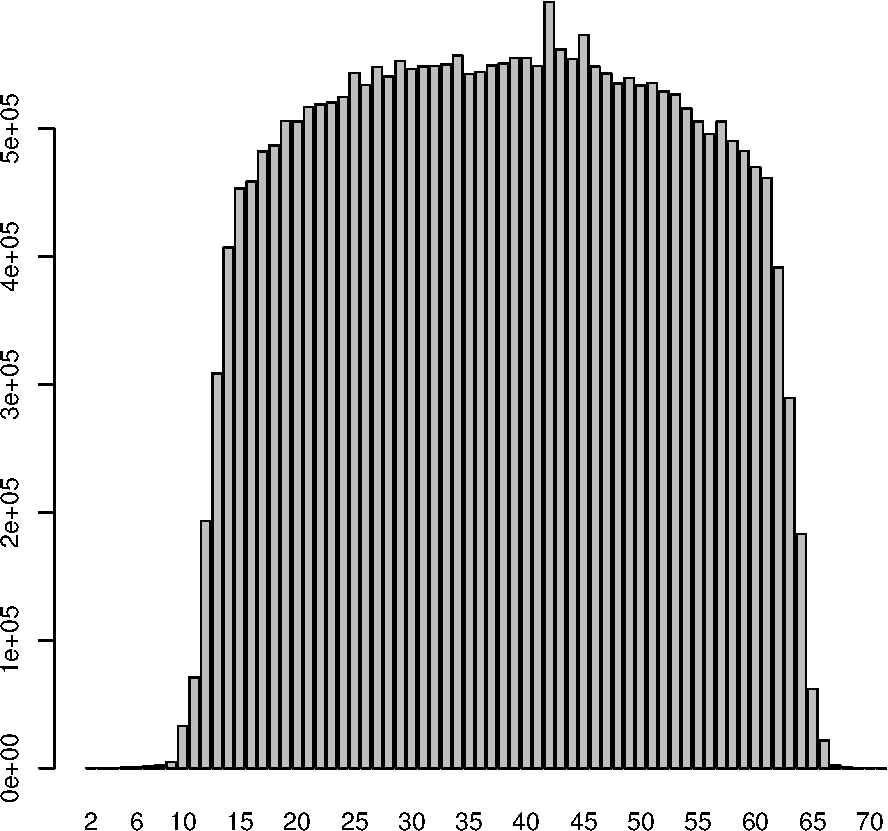
\includegraphics[width=0.5\textwidth]{latex/fig2_crop.pdf}}
\subfloat[Disproportion test\label{fig::qc2}]{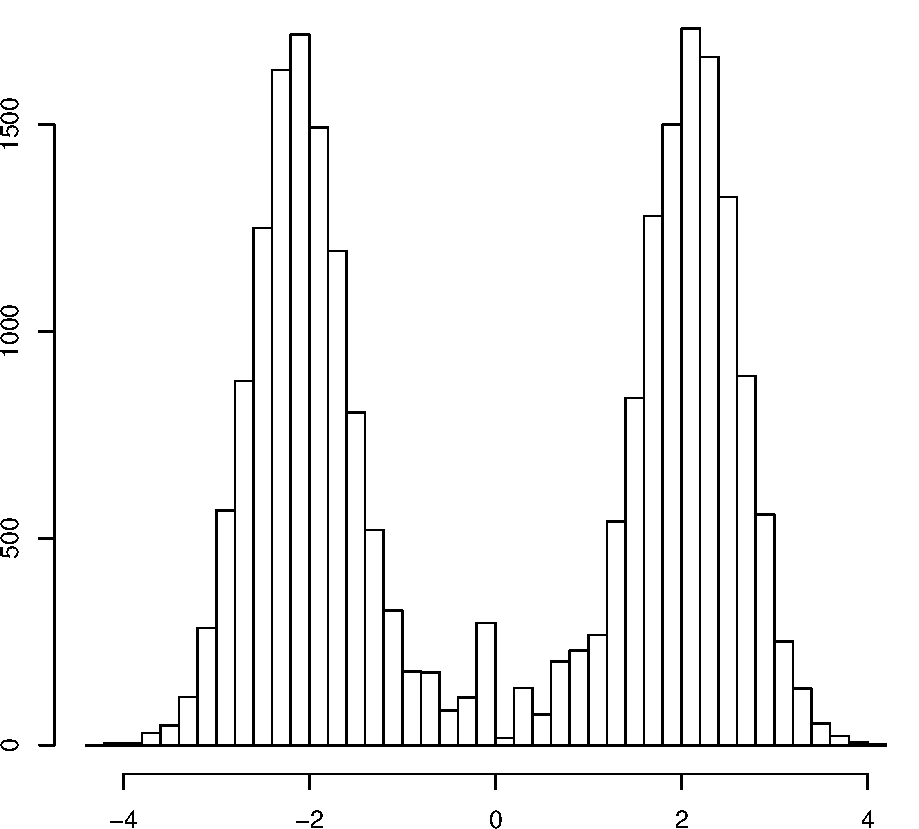
\includegraphics[width=0.5\textwidth]{latex/fig3_crop.pdf}}
\end{figure}

\subsection{Strand disproportion}
Another useful test is the distribution of $\log(c_+) - \log(c_-)$, where $c_+$ and $c_-$ are the number of counts on the plus and the minus strand, 
respectively. SJ with $c_+=0$ or $c_-=0$ are excluded. If the data is stranded and read1/read2 flags were set up correctly, then the distribution of
$\log(c_+) - \log(c_-)$ shall be bimodal as shown in Figure~\ref{fig::qc2}, reflecting the fact that one strand has much more split reads than 
the other.
\begin{verbatim}
Rscript disproportion.r <file.tsv> <file.pdf>
\end{verbatim}

\subsection{Summary stats on annotation status and splice sites}
As soon as splice junction counts are computed, it makes sense to ask what proportion of splice junctions is annotated and what is the distribution of
frequencies of splice site nucleotides. This is done by \prog{sjstat.r} utility.
\begin{verbatim}
R/sjstat.r <file.tsv>  >  <file.log>
\end{verbatim}

\bibliographystyle{plain}
\bibliography{sjpipeline}


\end{document}

